\ifpdf
	\graphicspath{{5/pic/PNG/}{5/pic/PDF/}{5/pic/}}
\else
	\graphicspath{{5/pic/EPS/}{5/pic/}}
\fi

\chapter{Neutronics modules for Hermes2D}\label{chap:hermes}

As we have seen in \cref{chap:nte-methods}, the various transport approximations lead to coupled systems of differential
equations with finite element approximations formulated on product spaces. In order to implement these models into a
practical solution method, it is thus neccessary to appropriately deal with the coupling of variables. 

In standard finite element
assembling procedures, we would need to use the same underlying mesh $\mesh$ and approximation space $\Space_{hp}$ for
all components of the solution (which, given the large differences in the behavior of the studied fields like group
fluxes, directional fluxes, or angular flux moments, means a significant waste of computational resources) or use some
form of data interpolation to evaluate integrals of type 
\begin{equation}\label{eq:mixed_int}
	\int_{\elem\in\mesh} \sigma_s^{gg'} u^g v^{g'}\,\d{\br}
\end{equation}
(as appearing for instance in the multigroup diffusion approximation) when $u^g$ and $v^{g'}$ do not live on the same
mesh. To avoid this interpolation and errors associated with it, the C++ finite element library Hermes2D uses the
original \textit{multimesh assembling} approach \cite{Hermes-thermoelasticity}. 

To illustrate Hermes2D capabilities for efficiently solving coupled PDE systems, we will consider the general form of
both the multigroup diffusion and $\SPN$ problems as discussed in \sref{sec:sp3_weak}, i.e. the general form of Problem
\ref{prb:sp3} (or, equivalently, \ref{prb:sp3bis}). As we are interested here in its finite element approximation, we
start by writing the restriction of this general weak problem to the approximation subspace constructed in such a
way that each component of the solution can be approximated by different set of basis functions:
$$ 
	\mathbb{V}_{hp} \equiv \mathbb{V}_{hp}(\VV) = \prod_{j=1}^M \Space_{j}^{hp}(\VV) \subset \mathbb{H}(\VV),
$$
where the component-specific spaces $\Space_{hp,j}$ will be substantiated below. 
\begin{problem}\label{prb:dif}
Given $\mathrm{Q} = \colset{q_i}{M} \in \left[\Lp[2](\VV)\right]^M$, find $\U_{hp} = \col \{u_{j}^{hp}\}_M \in
\mathbb{V}_{hp}$ such that
\begin{equation}\label{eq:weak_general}
\begin{gathered}
	a(\U_{hp}, \mathrm{V}) = f(\mathrm{V}) \quad \forall \mathrm{V}\in \mathbb{V}_{hp},\\[.3em]
	a(\mathrm{U}, \mathrm{V}) := \int_{\VV} \bigl(\mat{D}\nabla\mathrm{U} : \nabla \mathrm{V} +
	\mat{C} \mathrm{U}\cdot\mathrm{V}\bigr)\d{\br} +  \int_{\pV} \gamma\mat{G}\mathrm{U}\cdot\mathrm{V}
	\,\d{S},\\
 	f(\mathrm{V}) := \int_{\VV}\mathrm{Q}\cdot\mathrm{V}\,\d{\br},\quad \bigl(\mat{D}\nabla\mathrm{U}\bigr) : \nabla
 	\mathrm{V} = \sum_{j=1}^M\sum_{\alpha=1}^3 D_j\pd{u_j}{x_\alpha}\pd{v_j}{x_\alpha}
\end{gathered}
\end{equation}
where the diagonal matrix $\mat{D}$ and matrices $\mat{C}$ and $\gamma\mat{G}$ are defined in \eqref{eq:SP3_mat} and
Appendix \ref{app:SPN} for the  $\SPN[3,5,7]$ models and in \eqref{eq:dif_mat} for the multigroup diffusion ($\SPN[1]$)
model. As discussed in \sref{sec:sp3_weak}, eq. \eqref{eq:weak_general} can be put into an equivalent form \\[.2em]
\begin{equation*}
\begin{matrix}
		\a{1}{1} 	& + & \b{1}{2} 	& + & \cdots 	& + & \b{1}{M} 	& = & \l[1], &\ \forall v_1\in \Space_{1}^{hp}, \\[.25em]
		\b{2}{1} 	& + & \a{2}{2} 	& + & \cdots 	& + & \b{2}{M} 	& = & \l[2], &\ \forall v_2\in \Space_{2}^{hp}, \\[.25em]
		\vdots 		& 	& \vdots 		& 	&	\ddots	& 	&	\vdots 	 	& = & \vdots\\[.25em]
		\b{M}{1} 	& +	& \b{M}{2} 	& +	& \cdots 	& +	&	\a{M}{M} 	& = & \l[M], &\ \forall v_M\in \Space_{M}^{hp}
\end{matrix}
\end{equation*}\\[.2em]
where for $i,j = 1,2,\ldots, M$,\\[.2em]
\begin{equation*}
 	a_{ij}(u,v) := \int_{\VV} \bigl({D}_{ij}\nabla u \nabla v +
	C_{ij} u v \bigr)\d{\br} + \int_{\pV} \gamma G_{ij} u v
	\,\d{S},\quad
 	f_{i}(v) := \int_{\VV}q_i v\,\d{\br}.
\end{equation*}
\end{problem} 

\section{Multimesh hp-FEM}
\comment{
Consider the multi-group neutron diffusion problem in a typical thermal reactor with heterogeneous core.
As the neutron flux in lower energy groups (fast neutrons) is generally much smoother than flux in higher energy groups 
(slow neutrons), it makes sense to approximate each group on its own mesh and approximation space. Analogous situation 
arises in the mono-energetic $\SPN[5]$ problem -- as we will see in the examples below, the three $\SPN[5]$ moments 
$\phi^s_0$, $\phi^s_2$, $\phi^s_4$ generally behave very differently and the ability to approximate each moment 
independently can greatly save computational resources.} 



Let us define a set of meshes 
$$ \mesh^g = \{\elem^g\},\quad
	\overline{\VV} = \bigcup_{\elem^g\in\mesh^g} \overline\elem^g.
$$
We assume that the meshes originated from a common \textit{master mesh} $\mesh[h,m]$ by successive refinements
(independent for each mesh), but are otherwise arbitrary. The corresponding approximation
spaces are given by
\begin{equation}\label{eq:hermes_space}
	\Space_{hp}^g = \{v_{hp}^g \in C^0(\VV): \left. v_{hp}^g\right\vert_{\elem^g} \circ\, \mathfrak{r}^g \in
	\mathcal{P}_{p}(\hat{\elem}),\ \elem^g\in\mesh^g
	\}
\end{equation}
where $\hat{\elem}$ is the reference element (unit square or right triangle in Hermes2D), $\mathfrak{r}^g :
\elem^g \to \hat{\elem} $ maps the physical element in $g$-th mesh to the reference element and
$\mathcal{P}_{p}(\hat{\elem})$ is the space of polynomials of degree up to $p$ (tensor product polynomials in case of
$\elem$ being a quadrilateral). We will refer to the highest degree $p$ of the polynomial contained in the approximation
space as to the approximation order of that space. In Hermes2D, the meshes can contain both
triangular and quadrilateral elements. In order to prevent conditioning of the standard finite element stiffness matrices from blowing up with
increasing polynomial degree, hierarchical shape functions are used to construct the approximation spaces \eqref{eq:hermes_space} in
preference to the usual Lagrangian nodal basis (\cite[Sec. 2.5.3]{Hermes-book2}). In the case of a quadrilateral
mesh, for instance, $\Space_{hp}^g$ is composed of functions that are on the unit square $\hat\elem$
\begin{enumerate}
	\item[(a)] $p \geq 1$: bilinear functions with value $1$ in exactly one vertex of $\hat\elem$ and $0$
	in the remaining vertices,
	\item[(b)] $p \geq 2$: 2D polynomials with nonzero values on exactly one edge of $\hat\elem$ and vanishing on the
	remaining edges,
	\item[(c)] $p \geq 4$: 2D polynomials with nonzero values in the interior of $\hat\elem$ and vanishing on
	$\partial \hat\elem$.
\end{enumerate}
(see \fref{fig:bazep}).

\begin{figure}[!hb]
  \centering
  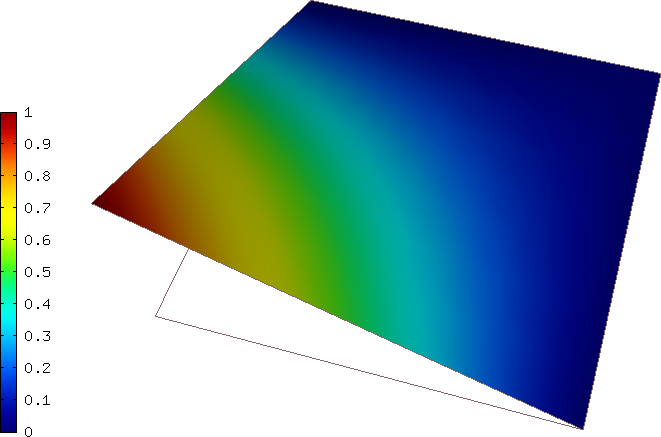
\includegraphics[width=.32\textwidth]{vtx}\hspace{.01\textwidth}
  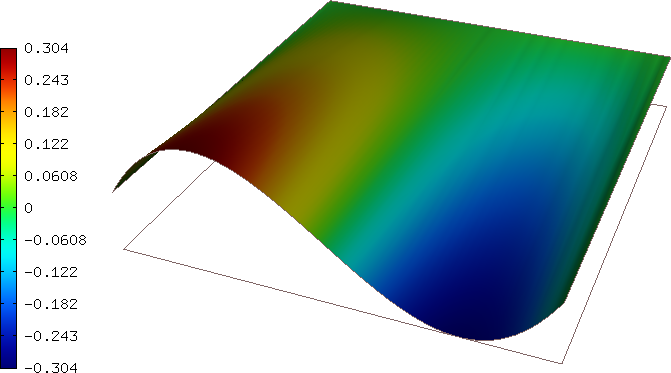
\includegraphics[width=.32\textwidth]{face}\hspace{.01\textwidth}
  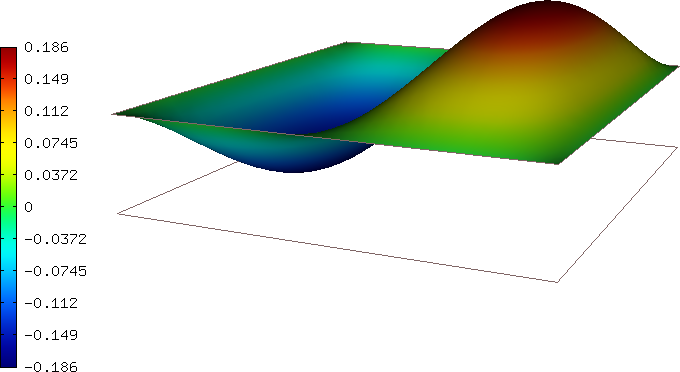
\includegraphics[width=.32\textwidth]{bubble}
  \caption{Shape functions of type (a), (b), (c).}
 	\label{fig:bazep}
\end{figure}

Note that the local approximation subspaces associated with each quadrilateral element might possess different
approximation orders in the lateral and longitudinal direction. Moreover, approximation orders may also vary from
element to element, i.e. for each $g$, $\Space_{hp}^g$ is decomposed into
\begin{equation}\label{eq:hermes_space}
	\Space_{hp,\tau}^g = \{v_{hp}^g \circ\, \mathfrak{r}^g \in
	\mathcal{P}_{p(\elem^g)}(\hat{\elem})
	\},\quad \elem^g\in\mesh^g,
\end{equation}
the local approximation subspaces constructed so that the minimum rule for $H^1$-conforming approximations
(\cite[\S3.5.5]{Hermes-book1}) -- namely that the approximation order of these subspaces coincides with the
approximation order in element interiors (thus constraining the polynomial degree of the edge shape functions during
assembling) -- is satisfied. We will henceofth identify an element with the local approximation subspace
constructed on top of it, so that we can speak of element orders, etc.

Lastly, hanging nodes (mesh vertices in edge interiors) are also
allowed in $\mesh^g$ for greater flexibility of mesh adaptivity (and $H^1$ conformity recovered by additional constraints on the edge shape functions as
described in \cite[\S3.6]{Hermes-book1} and \cite{Hermes-hanging-nodes}).

\subsection{Multimesh assembling}
We are now ready to describe the basic principle of the multimesh assembling algorithm. This has been nicely done in 
the original paper \cite{Hermes-thermoelasticity} (which we will closely follow) but we include the brief description
here as well as it is directly related to one of author's own contributions to Hermes2D described in
\sref{sec:hermes_dg}.

In order to assemble mixed integrals of type \eqref{eq:mixed_int}, the assembling procedure works with a geometrical union $\mesh[h,u]$ of all meshes $\mesh^1$, $\mesh^2$, $\mesh^3$. This union is never 
explicitly created in memory.
Rather, its virtual elements are traversed by the usual element-wise assembling loop. Let $\widetilde\elem \in \mesh[h,u]$
be the currently visited virtual element. As all meshes $\mesh^g$ originate from a common master mesh, there is for each
$g$ exactly one element $\elem^g\in\mesh^g$ such that $\widetilde\elem^g\subset \elem^g$ is the \textit{sub-element} of 
$\elem^g$ (which is called in this context the \textit{active element} on $\mesh^g$) corresponding to $\widetilde\elem$.
\begin{figure}[!hb]
  \centering
  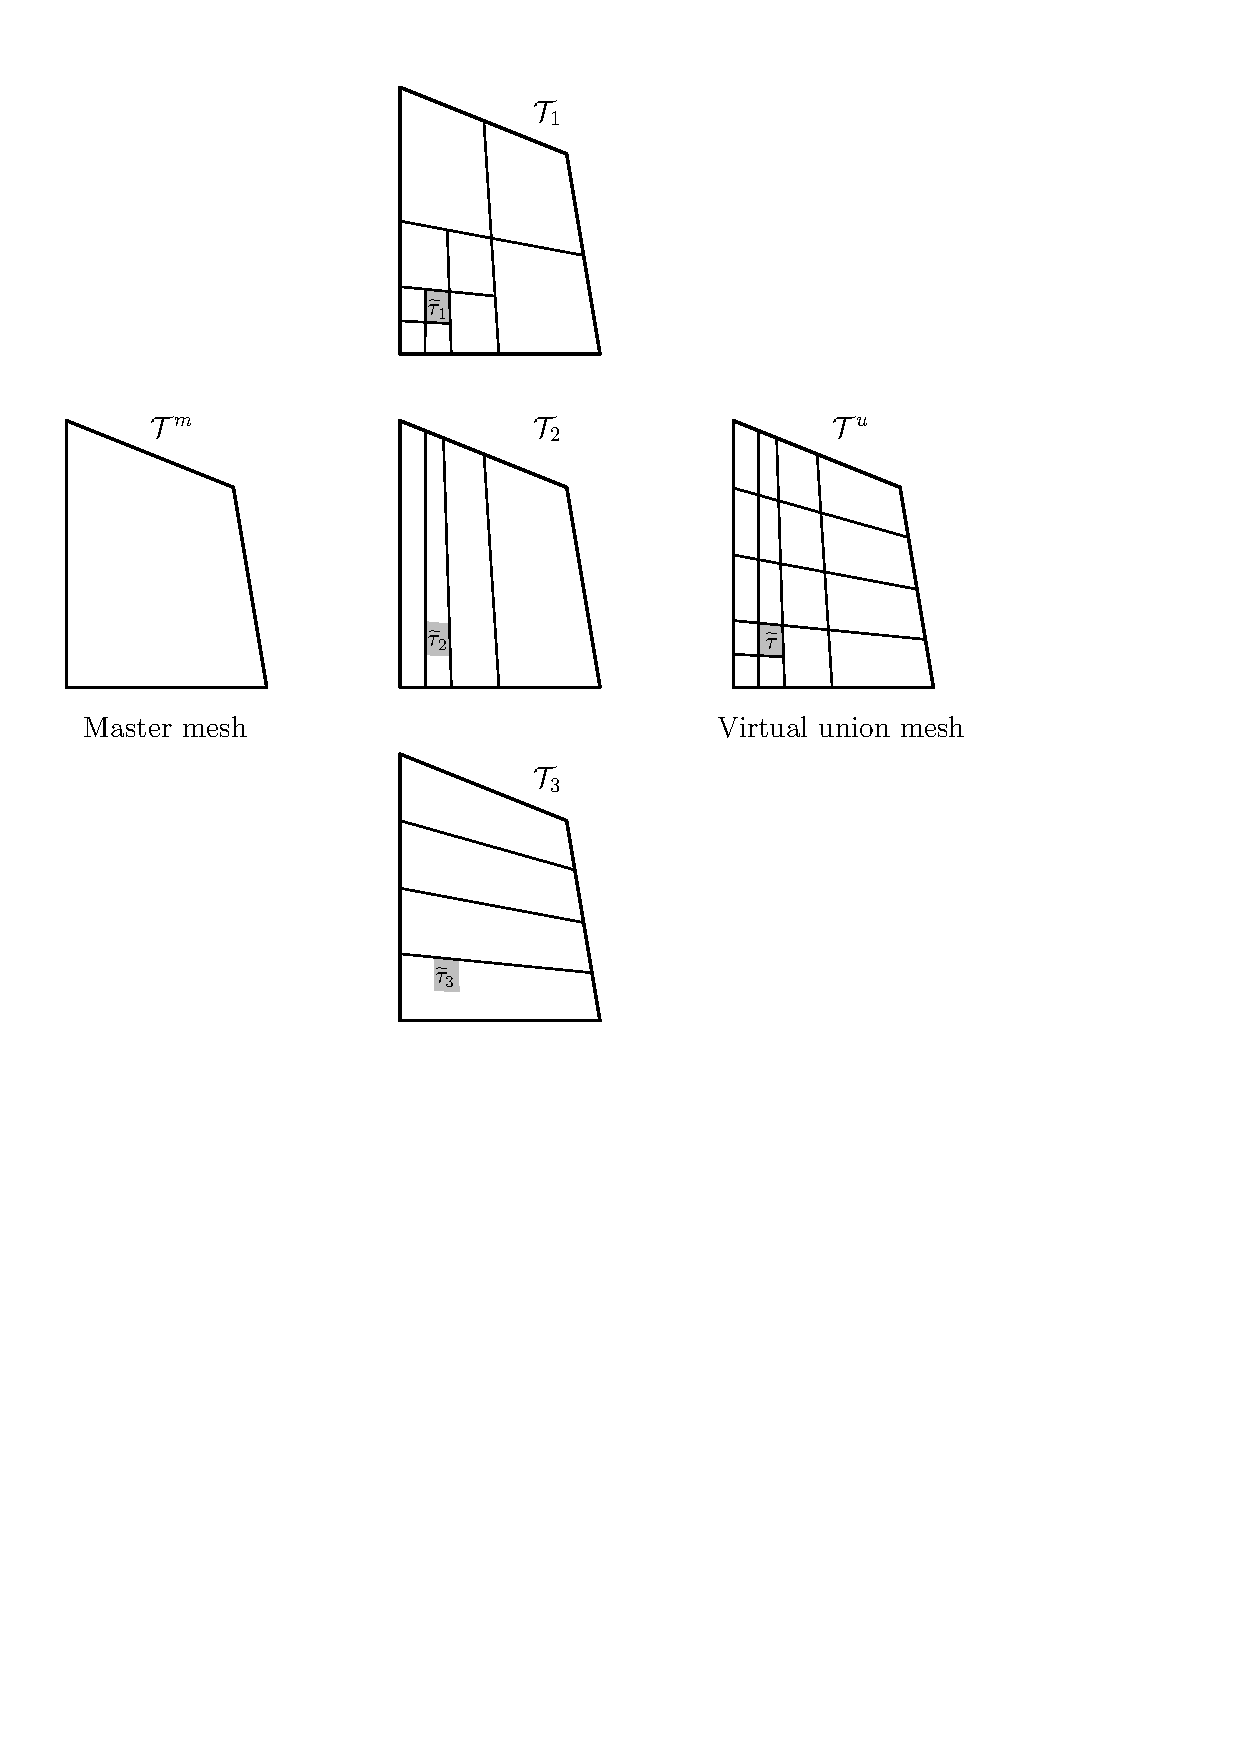
\includegraphics[scale=.9]{multimesh}
  \caption[Multimesh assembling]{One state of the multimesh assembling algorithm. Note that the sub-element mapping
  $\mathfrak{s}^1$ is identity.}
 	\label{fig:multimesh}
\end{figure}

To evaluate the integrals comprising the weak formulation of the problem (recall Prb. \ref{prb:sp3bis}), each
sub-element needs to be transformed to the reference element where the appropriate quadrature points are defined.
While for the active element on $\mesh^g$, the referece mapping $\mathfrak{r}^g(\elem^g) = \hat{\elem}$ as required, it
transforms the sub-element to a subset $\mathfrak{r}^g(\widetilde\elem^g) \subset \hat{\elem}$. Thus another mapping
$\mathfrak{s}^g : \hat{\elem} \to \hat{\elem}$ is introduced (the \textit{sub-element mapping}) such that
$\mathfrak{s}^g(\mathfrak{r}^g(\widetilde\elem^g)) = \hat{\elem}$. These two mappings allow Hermes2D to evaluate all
integrals in the weak forms by using elements only on the mesh on which the integrands live, thus incurring no further
error beyond the inevitable one of numerical integration.

\subsection{Discontinuous Galerkin assembling}\label{sec:hermes_dg}
As a joint effort of the author of this thesis and Luk{\' a}{\v s} Korous, at this moment (November 2014) the main
developer of the Hermes2D project, Hermes2D has been enabled for discontinuous Galerkin approximation of
variational problems. This involved the extension of the assembly procedure to
perform surface integration over all edges of all elements for user-defined discontinuous Galerkin bilinear and linear
forms and also exposing for these forms the access to shape functions and geometrical information of both elements sharing a
common interface (thus allowing the user to define interface operators like $\jump{\cdot}$ and $\langle\cdot\rangle$ introduced in
 \sref{sec:DGM}). 
 Because of the possibility of hanging nodes in the mesh (essentially needed for efficient mesh
 refinement), the actual integration of these forms along element edges is non-trivial as matching points
 from both sides of the edge need to be correctly determined.  
This functionality has been implemented in the class \lstinline{NeighborSearch} based on the same fundamental idea
underlying the multimesh assembling (namely that of sub-element mappings).

The \lstinline[basicstyle=\ttfamily]{NeighborSearch} class characterizes a neighborhood of a given edge in terms of adjacent
elements and provides methods for getting limit values of discontinuous functions from both sides of the edge. Each instance of the
class is connected to a mesh and its active element. The current active element becomes the \textit{central element} of
the neighborhood and all adjacent elements the \textit{neighbors}. In order to search for the neighboring elements, one
selects a particular edge of the central element and calls a function that enumerates the neighbors and fills in the
array of sub-element mappings (transformations) neccessary for getting function values at matching quadrature points
from both sides of the selected (active) edge.
The actual procedure depends on the relative size of the central element with respect to the neighbor element(s) across
the active edge:
\begin{itemize}
  \item If active edge is shared by two elements of same size, then the neighboring element is identified directly and 
  no additional transformations are needed to obtain values of any given function from either side of active edge.
\begin{figure}[!h]
  \centering
  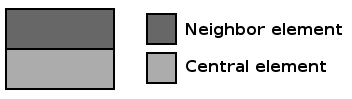
\includegraphics[scale=.45]{no_trans}
  \caption{Neighbor search -- ``no transformation'' case}
\end{figure}
  
  \item If the neighbor element is bigger than the central element, then we "go up" on the central element, until we
  find its parent that has the same size as the neighbor. We keep track of the visited intermediate parents and after 
  the final one has been found (in the ultimate case an element of the master
  mesh), we use them in reverse order to fill in the sub-element mapping array. These
  transformations will be applied to integration points used when integrating a function on the neighboring
  (bigger) element in order to obtain values at points matching those from the central element's side.
  
\begin{minipage}{\linewidth}
    \centering
    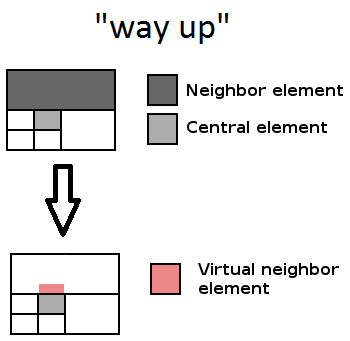
\includegraphics[scale=.6]{way_up2}
    \captionof{figure}{Neighbor search -- ``way up'' case}
\end{minipage}
  
  \item If the neighbor element is smaller than the central element, it means that it is one of several neighbors across
  the active edge. Hence, we "go down" in the central element in order to find a (virtual) sub-element matching the 
  currently processed neighbor and store the corresponding transformations in the neighbor's row of the
  (two-dimensional) array of sub-element mappings. This way, we obtain for each neighbor a set of
  transformations which will be applied on the central element to transform integration points to the correct
  sub-element matching the neighbor.

\begin{minipage}{\linewidth}
    \centering
    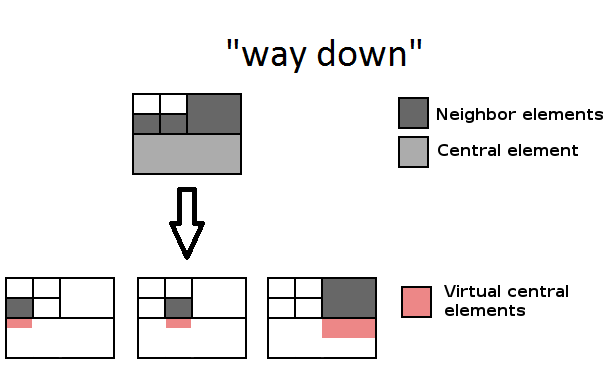
\includegraphics[scale=.6]{way_down2}
    \captionof{figure}{Neighbor search -- ``way down'' case}
\end{minipage}

\end{itemize}

If only an external function is supposed to be discontinuous across the active edge (e.g. in the case of assembling
linear forms), an appropriate \linebreak\lstinline[basicstyle=\ttfamily]{DiscontinuousFunc} object is created for such a
function and exposed to the user who can use it to retrieve actual values at the matching integration points from both
sides of the active segment.

If also the trial and test functions need to be considered discontinuous (e.g when assembling DG bilinear forms), the
local approximation bases (called \textit{shapesets} in Hermes2D) on the central element and on the current
neighbor element are extended by zero to the whole neighborhood of the two elements.
The so-called \textit{extended shapeset} thus created is 
queried during assembling for the count of all contained extended shape functions and their global DOF (degree of
freedom) numbers.
Assembling is done over all these extended shape functions -- the currently processed trial and test functions
is exposed to the user again as
\lstinline[basicstyle=\ttfamily]{DiscontinuousFunc} objects with the shape functions' values (and derivatives) at
integration points at both sides of active edge.
  
This procedure is limited by the requirement that the number of integration points at both sides of
active edge is the same. This is enforced artificially during assembling by performing the integrations of DG interface
forms using a quadrature of the maximal supported order. Note that this does not restricts the approximation spaces
in any way -- it only pertains to the numerical integration.

\section{$hp$-adaptivity}\label{sec:hermes_adapt}
The goal of the $hp$-adaptivity process is to combine spatial subdivision of selected elements ($h$-refinement) with
local increase of their approximation order ($p$-refinement) so that the total available number of degrees of freedom at given stage of
the process is utilized most efficently (i.e., relatively big number of low-order elements is used in regions with highly oscillating solution
while smaller number of high-order elements in regions with smoother solution behavior). As there are many
possible combinations of $h$ and $p$ refinements of given element, one number per element provided by traditional
a-posteriori error estimates for FEM is insufficient to guide the $hp$ adaptivity. Instead, a robust
approach to local error estimation is used in Hermes2D that is based on comparing two
solutions of different approximation orders (note that this technique has been used for a long time for solving the
ordinary differential equations). This allows to determine the whole shape of the approximation error $e = u - u_{hp}$ 
over each element and use it to determine the best refinement candidate that decreases the total approximation error for
the lowest number of added DOF. 

For illustration, let us consider the general approximate problem \ref{prb:general}, coming from the corresponding
exact variational problem with solution $\U\in\mathbb{H}^1(\VV)$.

To understand the $hp$-adaptivity algorithm in the multimesh setting, we must realize that the approximation error is a
vector field with components corresponding to  is characterized by the following steps (which will be commented in more
detail below)

\begin{enumerate}
	\item approximate $\flfl$ on current set of spaces $\Space_{hp}^g$ to obtain $\flfl_{hp}$
	\item global refinement: $\Space_{hp}^g \to \Space_{h/2,p+1}^g$, obtain $\flfl_{h/2,p+1}$
	\item set $\flfl_{\rf} = \flfl_{h/2,p+1}$, compute $\indic^g_\elem = \norm[\elem,g]{\fl_{hp}^g-\fl^g_{\rf}}^2$ for
	each element $\elem^g \in \mesh^g$; here  
	\item accumulate $\indic_{hp,\elem}^g$ from all meshes $\tau^g$ to obtain
	$E_{hp}=\tzterm{norm}{\norm{\flfl_{hp}-\flfl_{\rf}}}$ ~~\gray{\footnotesize (note that $\norm{E_{hp}}^2 = \sum_g\sum_{K_n^g\in\tau^g}\indic^g_n$ where $\indic^g_n = \norm[n,g]{\fl_{hp}^g-\fl^g_{\rf}}^2$)}
	%                \gray{\footnotesize (by accumulating error estimates from all $K_n^g\in\tau^g$)}
	\item stop if $\frac{E_{hp}}{\norm{\flfl_{\rf}}} \leq TOL$, otherwise
	\item mark elements $K_n^g$ for which $\frac{\indic^g_n}{\tzterm{normelem}{\norm[n,g]{\fl_{\rf}^g}}} > \theta\max_{n',g'}\frac{\indic^{g'}_{n'}}{\norm[n',g']{\fl_{\rf}^{g'}}}$
	\item decide refinement strategy ($h$-, $p$-, iso/anisotropic, etc.)  
	\item refine marked elements ($\Space_{hp}^g \to V_{h'p'}^g$)
\end{enumerate}

Note that $\indic_g$ 